% Provenance (never printed): old premiere S material on subduction (Wadati-Benioff
% planes, density of the old lithosphere, slab pull, transformation of the slab at
% depth: blueschist and eclogite; anatomy of an active margin). Sections from
% figdata/grade-11/slab_sections.py (USGS ComCat M >= 6 1976-2025, PB2002 steps,
% Seton 2020 ages); plate speeds from plate_velocities.py (NNR-MORVEL56 RMS).
% Metamorphism is defined in g12.03, the volcanic arc in g12.04: named only here.
\chapter{Les zones de subduction}\label{ch:g11:subduction-zones}

Sous les îles Tonga, dans le sud-ouest du Pacifique, la Terre tremble bien
plus profondément que partout ailleurs. Sur les sept mille séismes de
magnitude 6 ou plus enregistrés dans le monde entre 1976 et 2025, le plus
profond s'est produit à \qty{688}{km}, et la coupe des Tonga présentée dans
ce chapitre contient des événements jusque vers \qty{671}{km}. À de telles
profondeurs, la roche est chaude et soumise à une pression énorme~; elle
devrait s'écouler lentement, comme l'\omterm{def:g11:lithosphere-asthenosphere:lithosphere}{asthénosphère}, et non se rompre. Elle
se rompt pourtant. Ce chapitre explique ce qui s'y trouve pour se rompre~:
un \omterm{def:g11:subduction-zones:slab}{panneau} de fond océanique froid qui replonge dans le manteau.
% ledger: data:usgs-comcat (catalogue_maxdepth 688; tonga_maxdepth 670.8, slab_sections.py)

\begin{recall}
À une limite convergente, deux plaques se rapprochent l'une de l'autre~; des
fosses profondes bordent certaines d'entre elles (livre~1, années~7 et~8).
La magnitude d'un séisme mesure sa taille, et un séisme sous la mer peut
déclencher un tsunami (livre~1, année~7). La vitesse d'une plaque par
rapport à une autre est la différence de leurs vitesses
(\cref{ch:g11:plate-motions}). Le fond océanique s'enfonce en vieillissant,
et après quelque 60 millions d'années sa \omterm{def:g11:lithosphere-asthenosphere:lithosphere}{lithosphère}, épaisse d'environ
\qty{100}{km}, est plus dense que l'\omterm{def:g11:lithosphere-asthenosphere:lithosphere}{asthénosphère} située dessous
(\cref{ch:g11:ocean-ridges}). Les ondes sismiques révèlent un changement
brusque dans le manteau vers \qty{670}{km} (\cref{ch:g11:seismic-structure}).
Une roche métamorphique est une roche transformée à l'état solide (livre~1,
année~6).
\end{recall}
% ledger: data:prem (670 km), ps77:depth-age

\section{Fosses et zones de séismes inclinées}

La plupart des séismes sont superficiels~: dans le catalogue des séismes de
magnitude 6 ou plus depuis 1976, environ un sur cinq seulement se produit à
plus de \qty{70}{km} de profondeur, et un sur quinze à plus de
\qty{300}{km}. La carte ci-dessous montre où se trouvent les plus profonds.
% values (slab_sections.py): frac_deeper_70 0.21, frac_deeper_300 0.069; data:usgs-comcat

\begin{omfigure}
\begin{tikzpicture}
\begin{axis}[ommap, width=\linewidth, xtick={-180,-90,...,180}, ytick={-60,0,60},
  legend style={font=\scriptsize, at={(0.5,-0.13)}, anchor=north, legend columns=3,
    /tikz/every even column/.append style={column sep=6pt}}]
\addplot[fill=omLithAlluv, draw=black!45, line width=0.2pt, forget plot] table {figdata/out/shared-geo-land.dat};
\addplot[black!70, line width=0.5pt, forget plot] table {figdata/out/shared-geo-school-subduction.dat};
\addplot[fill=black!70, draw=none, forget plot] table {figdata/out/shared-geo-school-teeth.dat};
% computed in figdata/grade-11/slab_sections.py; ledger: data:usgs-comcat, data:pb2002
\addplot[only marks, mark=*, mark size=0.55pt, black!45] table[x=lon, y=lat] {figdata/out/grade-11-slab_sections-world-shallow.dat};
\addplot[only marks, mark=*, mark size=0.8pt, omProp] table[x=lon, y=lat] {figdata/out/grade-11-slab_sections-world-mid.dat};
\addplot[only marks, mark=*, mark size=1.1pt, omThm] table[x=lon, y=lat] {figdata/out/grade-11-slab_sections-world-deep.dat};
\legend{{moins de \qty{70}{km} de profondeur}, {70 à \qty{300}{km}}, {plus de \qty{300}{km} de profondeur}}
\end{axis}
\end{tikzpicture}

{\small Séismes de magnitude 6.5 ou plus, 1976--2025 (2192 événements),
colorés selon leur profondeur, avec les fosses (trait noir, triangles sur la
plaque chevauchante). Les séismes intermédiaires et profonds ne se trouvent
que le long de certaines fosses, toujours du côté de la plaque chevauchante.
Données~: catalogue des séismes de l'USGS~; limites de plaques de Bird
(2003)~; terres émergées~: Natural Earth.}
\end{omfigure}
% values: world_n_m65 2192, world_deep_n 197 (slab_sections.py)

Les séismes profonds ne sont pas dispersés~: ils suivent les fosses du
Pacifique Ouest, du Kamtchatka au Japon, aux Mariannes, à l'Indonésie et aux
Tonga, ainsi que la fosse qui longe la côte ouest de l'Amérique du Sud~; et
ils se trouvent toujours d'un même côté de la fosse, sous la plaque qui ne
s'enfonce pas.

\begin{definition}[Subduction~; zone de subduction]\label{def:g11:subduction-zones:subduction}
La \emph{subduction}\index{subduction} est l'enfoncement d'une plaque de
\omterm{def:g11:ocean-ridges:oceanic-lithosphere}{lithosphère océanique} sous une autre plaque, qui la ramène dans le manteau.
Une \emph{zone de subduction}\index{zone de subduction} est une limite de
plaques convergente où se produit une subduction~; elle est marquée en
surface par une fosse.
\end{definition}

\begin{definition}[Zone de Wadati--Benioff]\label{def:g11:subduction-zones:benioff}
Une \emph{zone de Wadati--Benioff}\index{zone de Wadati--Benioff} est la
bande inclinée de séismes qui part d'une fosse et s'enfonce de plus en plus
sous la plaque chevauchante, jusqu'à environ \qty{700}{km} de profondeur au
plus.
\end{definition}
% ledger: frohlich87:wadati

\begin{history}[Wadati et Benioff]
Dans les années 1920, d'éminents sismologues soutenaient que les séismes ne
pouvaient se produire que dans les premières dizaines de kilomètres~: la
Terre profonde, pensaient-ils, n'avait pas la résistance nécessaire pour
accumuler la déformation. Le sismologue japonais Kiyoo Wadati, qui
travaillait avec le réseau dense de stations de l'Agence météorologique du
Japon, apporta à partir de 1928 la première preuve convaincante que certains
séismes se produisent à des centaines de kilomètres de profondeur~: l'un des
événements qu'il étudia, en janvier 1927, s'était produit à \qty{420}{km}.
En 1935, il publia la première carte des profondeurs de ces séismes,
tracée en courbes de niveau, et remarqua que la zone qui s'enfonce était
parallèle à l'alignement des volcans actifs. En 1949 et en 1954, le
sismologue américain Hugo Benioff montra que, sous les Andes et sous les
îles Tonga--Kermadec, les séismes s'alignent le long de zones qui atteignent
environ \qty{700}{km} de profondeur. Ces zones furent d'abord appelées zones
de Benioff, en 1967~; le nom de \omterm{def:g11:subduction-zones:benioff}{zone de Wadati--Benioff}, qui rend justice
aux deux, suit une proposition du géophysicien japonais Seiya Uyeda en 1971.
\end{history}
% ledger: frohlich87:wadati

\begin{method}[Lire une coupe de séismes]\label{met:g11:subduction-zones:section}
\begin{enumerate}
  \item Choisir une ligne perpendiculaire à la fosse, allant de la fosse
        vers la plaque chevauchante, et garder les séismes situés dans une
        bande de part et d'autre de cette ligne.
  \item Placer chaque séisme à sa distance le long de la ligne
        (horizontalement) et à sa profondeur (verticalement, vers le bas).
  \item Chercher la bande inclinée~; tracer la droite qui la suit le mieux.
  \item Lire le pendage de la bande à partir de deux points de la droite
        (proposition ci-dessous).
\end{enumerate}
\end{method}

\begin{omfigure}
\begin{tikzpicture}
\begin{axis}[omrecord, omdepth, name=tonga, width=0.5\linewidth, height=6.4cm,
  xmin=-150, xmax=900, ymin=0, ymax=720, xlabel={distance à la fosse (\unit{km})},
  ylabel={profondeur (\unit{km})}, title={\small Tonga}, clip=false]
% computed in figdata/grade-11/slab_sections.py; ledger: data:usgs-comcat, data:pb2002
\addplot[only marks, mark=*, mark size=1.2pt, black!65] table[x=x, y=depth] {figdata/out/grade-11-slab_sections-tonga.dat};
\addplot[omProp, line width=1pt, domain=135.7:761.6, samples=2] {-23.568 + 0.91068*x};
\addplot[only marks, mark=triangle*, mark size=3pt, omDef] coordinates {(0,0)};
\node[font=\scriptsize, anchor=south west, text=omDef] at (axis cs:10,8) {fosse};
\node[font=\scriptsize, anchor=west, text=omProp, align=left] at (axis cs:300,560) {pendage\\\ang{42}};
\end{axis}
\begin{axis}[omrecord, omdepth, at={(tonga.east)}, anchor=west, xshift=0.3cm, width=0.5\linewidth, height=6.4cm,
  xmin=-150, xmax=900, ymin=0, ymax=720, xlabel={distance à la fosse (\unit{km})},
  yticklabels={}, title={\small Andes, vers \ang{21} Sud}, clip=false]
\addplot[only marks, mark=*, mark size=1.2pt, black!65] table[x=x, y=depth] {figdata/out/grade-11-slab_sections-andes.dat};
\addplot[omProp, line width=1pt, domain=253.0:900, samples=2] {-88.745 + 0.74613*x};
\addplot[only marks, mark=triangle*, mark size=3pt, omDef] coordinates {(0,0)};
\node[font=\scriptsize, anchor=south west, text=omDef] at (axis cs:10,8) {fosse};
\node[font=\scriptsize, anchor=west, text=omProp, align=left] at (axis cs:300,560) {pendage\\\ang{37}};
\end{axis}
\end{tikzpicture}

{\small Coupes de séismes perpendiculaires à deux fosses~: séismes de
magnitude 6 ou plus, 1976--2025, situés à moins de \qty{150}{km} de la ligne
de coupe, placés selon leur distance à la fosse (vers la plaque
chevauchante) et leur profondeur. En orange~: la droite qui suit le mieux
les séismes situés entre 100 et \qty{600}{km} de profondeur. Sous les
Tonga, la bande descend au-delà de \qty{670}{km}. Données~: catalogue des
séismes de l'USGS~; positions des fosses d'après Bird (2003).}
\end{omfigure}
% values (slab_sections.py): tonga_dip 42.3, fit -23.568 + 0.91068 x (77 events);
% andes_dip 36.7, fit -88.745 + 0.74613 x; trench points tonga (-173.31, -20.395),
% andes (-71.286, -21.01)

\begin{proposition}[Le pendage d'un panneau plongeant d'après une coupe de séismes]\label{prop:g11:subduction-zones:dip}
Si deux points de la droite qui suit une \omterm{def:g11:subduction-zones:benioff}{zone de Wadati--Benioff} se trouvent
aux distances horizontales $x_1 < x_2$ de la fosse et aux profondeurs $z_1$
et $z_2$, son pendage $\delta$, l'angle qu'elle fait avec l'horizontale,
vérifie
\[
  \tan \delta = \frac{z_2 - z_1}{x_2 - x_1}.
\]
\end{proposition}

\begin{proof}
Les deux points et le point situé à la profondeur $z_1$ à la verticale du
second forment un triangle rectangle. Son côté horizontal vaut $x_2 - x_1$,
son côté vertical $z_2 - z_1$, et l'angle au premier point est le pendage.
La tangente d'un angle d'un triangle rectangle est le rapport du côté
opposé au côté adjacent.
\end{proof}

\begin{example}[Le pendage sous les Tonga]\label{ex:g11:subduction-zones:dip}
La droite de la coupe des Tonga passe à \qty{250}{km} de profondeur à
\qty{300}{km} de la fosse et à \qty{614}{km} de profondeur à
\qty{700}{km}. Donc
$\tan\delta = (614 - 250)/(700 - 300) = 364/400 = 0.91$, et
$\delta \approx \ang{42}$. Sous les Andes, à \ang{21}~Sud, la même méthode
donne environ \ang{37}.
\end{example}
% values: tonga line at 300 km 249.6, at 700 km 613.9 (slab_sections.py)

La \omterm{def:g11:subduction-zones:benioff}{zone de Wadati--Benioff} dessine une plaque qui descend. Les séismes
superficiels se produisent là où les deux plaques frottent l'une contre
l'autre, près de la fosse~; les plus profonds se produisent à l'intérieur
même de la plaque qui s'enfonce.

\section{Pourquoi la lithosphère ancienne s'enfonce}

\begin{definition}[Panneau plongeant]\label{def:g11:subduction-zones:slab}
Un \emph{panneau plongeant}\index{panneau plongeant} est la partie d'une
plaque qui s'est déjà enfoncée dans le manteau à une \omterm{def:g11:subduction-zones:subduction}{zone de subduction}~:
une lame de \omterm{def:g11:ocean-ridges:oceanic-lithosphere}{lithosphère océanique}, épaisse d'une centaine de kilomètres,
inclinée sous la plaque chevauchante.
\end{definition}

Ce qui descend, c'est du fond océanique ancien. D'après l'âge du fond
océanique, le fond qui atteint la fosse du Japon, à l'est du Japon, a
environ 133 millions d'années, celui qui atteint la fosse des Tonga environ
99 millions d'années~; même le fond qui atteint les Andes, l'un des plus
jeunes à s'enfoncer, a environ 49 millions d'années. Une \omterm{def:g11:lithosphere-asthenosphere:lithosphere}{lithosphère} aussi
ancienne est froide et épaisse et, à part sa croûte légère, plus dense que
l'\omterm{def:g11:lithosphere-asthenosphere:lithosphere}{asthénosphère}~: dès qu'un de ses bords commence à descendre, son propre
poids l'entraîne.
% values (slab_sections.py): japan_age 133.1, tonga_age 98.8, andes_age 48.8 (median of the
% 1-degree cells 100-400 km seaward of the trench point); ledger data:b2-seafloor-age

\begin{definition}[Traction du panneau plongeant~; poussée à la dorsale]\label{def:g11:subduction-zones:slab-pull}
La \emph{traction du panneau plongeant}\index{traction du panneau plongeant}
est la force qu'un \omterm{def:g11:subduction-zones:slab}{panneau plongeant}, plus dense que le manteau qui
l'entoure, exerce sur le reste de sa plaque, en la tirant vers la fosse. La
\emph{poussée à la dorsale}\index{poussee a la dorsale@poussée à la dorsale}
est la force qui éloigne une plaque d'une dorsale, là où la
\omterm{def:g11:lithosphere-asthenosphere:lithosphere}{lithosphère} jeune et chaude se tient haut sur le relief de la dorsale et
glisse le long de sa pente.
\end{definition}

Laquelle des deux compte le plus~? En 1975, Donald Forsyth et Seiya Uyeda
évaluèrent l'intensité de chaque force à partir des vitesses et des formes
des plaques~: les forces qui s'exercent sur les \omterm{def:g11:subduction-zones:slab}{panneaux plongeants}
contrôlent la vitesse des plaques océaniques, et sont environ dix fois plus
intenses que toute autre force. Les vitesses actuelles des plaques le
montrent clairement.
% ledger: fu75:slab-pull

\begin{omfigure}
\begin{tikzpicture}
\begin{axis}[omrecord, ybar, bar width=9pt, width=0.86\linewidth, height=5.6cm,
  ymin=0, ymax=85, xmin=-0.7, xmax=12.7, bar shift=0pt, ylabel={vitesse moyenne (\unit{mm} par an)},
  xtick={0,...,12}, xticklabel style={rotate=50, anchor=east, font=\scriptsize},
  xticklabels={Cocos, Nazca, Pacifique, Australie, mer des Philippines, Arabie, Somalie,
    Nubie, Eurasie, Amérique du Nord, Antarctique, Caraïbes, Amérique du Sud},
  ymajorgrids, xmajorgrids=false]
% computed in figdata/grade-11/slab_sections.py from plate_velocities.POLES (nnr56:rms)
\addplot[fill=omProp, draw=omProp!70!black] table[x=idx, y expr=\thisrow{slab}*\thisrow{rms}] {figdata/out/grade-11-slab_sections-speeds.dat};
\addplot[fill=omDef!35, draw=omDef] table[x=idx, y expr=(1-\thisrow{slab})*\thisrow{rms}] {figdata/out/grade-11-slab_sections-speeds.dat};
\node[font=\scriptsize, text=omProp!80!black, anchor=south] at (axis cs:2,76) {panneau plongeant attaché};
\node[font=\scriptsize, text=omDef, anchor=south] at (axis cs:9,50) {pas de long panneau plongeant};
\end{axis}
\end{tikzpicture}

{\small La vitesse moyenne de treize grandes plaques (moyenne quadratique
sur la plaque, dans un référentiel dans lequel la \omterm{def:g11:lithosphere-asthenosphere:lithosphere}{lithosphère} dans son
ensemble ne tourne pas). En orange~: les plaques auxquelles pend un \omterm{def:g11:subduction-zones:slab}{panneau
plongeant} le long d'une grande partie de leur bord~; en bleu~: les plaques
qui n'en ont pas. L'Inde est laissée de côté~: son bord nord est une
collision. Données~: NNR-MORVEL56 (Argus, Gordon et DeMets, 2011).}
\end{omfigure}
% ledger: nnr56:rms; the bars of a class are drawn at 0 for the other (two series on one axis)

\begin{proposition}[Les plaques attachées à des panneaux plongeants sont rapides]\label{prop:g11:subduction-zones:fast}
Les cinq grandes plaques auxquelles pend un long \omterm{def:g11:subduction-zones:slab}{panneau plongeant} (Cocos,
Nazca, Pacifique, Australie, mer des Philippines) se déplacent en moyenne à
environ \qty{65}{mm} par an~; les huit qui n'en ont pas, à environ
\qty{24}{mm} par an, près de trois fois plus lentement. Chaque plaque du
premier groupe est plus rapide que toutes les plaques du second.
\end{proposition}
% values: rms_slab_mean 65.2, rms_noslab_mean 23.9 (plate_velocities.py); India left out
% (its northern edge is a collision)

\begin{proof}
D'après les vitesses moyennes publiées, les plaques à \omterm{def:g11:subduction-zones:slab}{panneau plongeant}
donnent
$(74.6 + 70.0 + 65.5 + 63.1 + 52.6)/5 \approx 65.2$ et les autres
$(47.6 + 31.0 + 29.2 + 22.8 + 19.8 + 15.2 + 14.9 + 10.6)/8 \approx 23.9$
(millimètres par an)~; la plus lente des plaques à \omterm{def:g11:subduction-zones:slab}{panneau plongeant}, la
plaque de la mer des Philippines à 52.6, est plus rapide que la plus rapide
des autres, l'Arabie à 47.6.
\end{proof}
% ledger: nnr56:rms

\section{Le panneau plongeant transformé en profondeur}

À mesure que le \omterm{def:g11:subduction-zones:slab}{panneau plongeant} descend, sa croûte de basalte et de \omterm{def:g11:ocean-ridges:gabbro}{gabbro}
est enfouie de plus en plus profondément tout en restant froide, car le
\omterm{def:g11:subduction-zones:slab}{panneau} s'enfonce plus vite que la chaleur ne peut atteindre son intérieur.
Les roches de la croûte changent de minéraux sans fondre~: elles sont
métamorphisées (\cref{ch:g12:metamorphic-rocks}). Deux roches jalonnent le
trajet.

\begin{definition}[Schiste bleu~; éclogite]\label{def:g11:subduction-zones:eclogite}
Le \emph{schiste bleu}\index{schiste bleu} est une roche métamorphique issue
du basalte de la \omterm{def:g11:ocean-ridges:oceanic-lithosphere}{croûte océanique} enfoui à haute pression tout en restant
relativement froid~; il doit sa couleur bleue à un minéral, la glaucophane.
L'\emph{éclogite}\index{eclogite@éclogite} est la roche métamorphique dense
que deviennent le basalte et le \omterm{def:g11:ocean-ridges:gabbro}{gabbro} aux profondeurs du manteau le long
des \omterm{def:g11:subduction-zones:subduction}{zones de subduction}~: elle a la même composition chimique, mais elle
est faite de grenat rouge et de pyroxène vert.
\end{definition}
% ledger: photo:g11-blueschist, photo:g11-eclogite

\begin{omfigure}
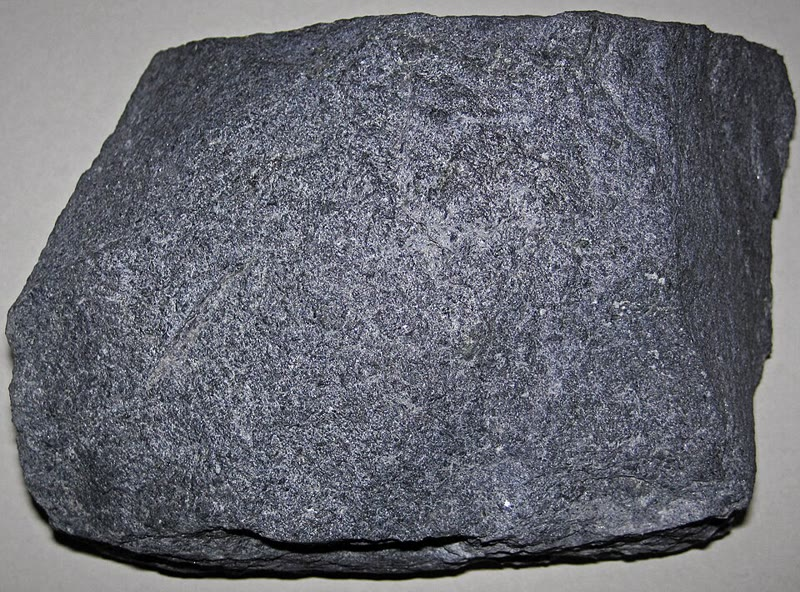
\includegraphics[height=4.4cm]{images/book2/g11-stjohn-blueschist.jpg}\hspace{0.03\linewidth}%
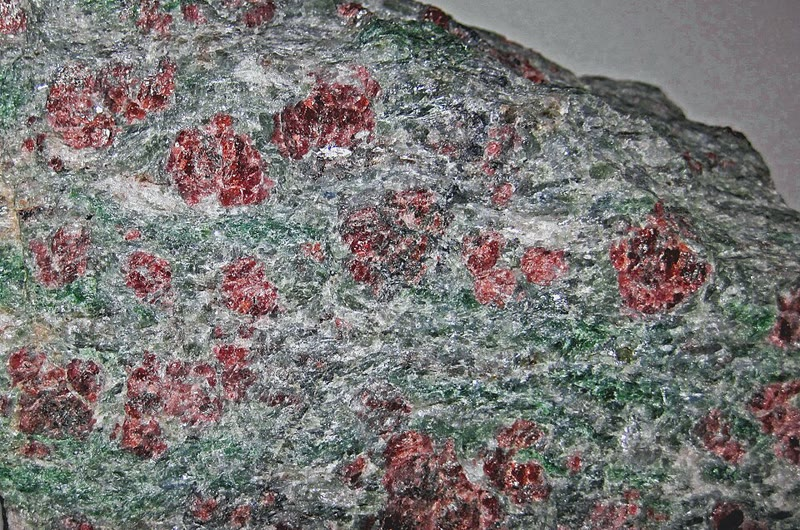
\includegraphics[height=4.4cm]{images/book2/g11-stjohn-eclogite.jpg}

{\small À gauche~: un \omterm{def:g11:subduction-zones:eclogite}{schiste bleu} de l'île Santa Catalina, en Californie,
ancienne \omterm{def:g11:ocean-ridges:oceanic-lithosphere}{croûte océanique} enfouie dans une \omterm{def:g11:subduction-zones:subduction}{zone de subduction}. À droite~:
une \omterm{def:g11:subduction-zones:eclogite}{éclogite} de Norvège, avec des grenats rouges dans du pyroxène vert.
Photographies James St.~John (CC~BY~2.0).}
\end{omfigure}
% ledger: photo:g11-blueschist, photo:g11-eclogite

L'\omterm{def:g11:subduction-zones:eclogite}{éclogite} est plus dense que le basalte~; elle est même plus dense que la
\omterm{def:g11:ocean-ridges:peridotite}{péridotite} du manteau, d'environ \qty{6}{\percent}. Une fois sa croûte
transformée en \omterm{def:g11:subduction-zones:eclogite}{éclogite}, le \omterm{def:g11:subduction-zones:slab}{panneau plongeant} ne porte plus de couche
légère à son sommet~: tout le \omterm{def:g11:subduction-zones:slab}{panneau} est plus dense que le manteau qui
l'entoure, et il tire plus fort. Les roches de ce type, ramenées à la
surface par des mouvements ultérieurs, font partie des rares témoins
directs de ce qui se passe à des dizaines de kilomètres de profondeur dans
une \omterm{def:g11:subduction-zones:subduction}{zone de subduction}.
% ledger: hacker03:eclogite, photo:g11-eclogite

\begin{omfigure}
\begin{tikzpicture}[font=\footnotesize, scale=0.85]
  % subduction zone, a drawing, not to scale: slab top flat to x = -1, then bends to a 42-degree dip
  % coordinates computed once by a small script (scratch, not kept): slab top flat to x=-1, arc R=3 to a 42-degree dip
  \fill[omProp!10] (-7,-1.4) rectangle (7,-6.0);
  \fill[omSea!45] (-7,0) -- (-1,0) -- (1.6,0.8) -- (-7,0.8) -- cycle;
  \fill[lith peridotite] (-7.000,0.000) -- (-6.644,0.000) -- (-6.289,0.000) -- (-5.933,0.000) -- (-5.578,0.000) -- (-5.222,0.000) -- (-4.867,0.000) -- (-4.511,0.000) -- (-4.156,0.000) -- (-3.800,0.000) -- (-3.445,0.000) -- (-3.089,0.000) -- (-2.734,0.000) -- (-2.378,0.000) -- (-2.023,0.000) -- (-1.667,0.000) -- (-1.312,0.000) -- (-0.956,-0.000) -- (-0.602,-0.027) -- (-0.253,-0.094) -- (0.085,-0.203) -- (0.408,-0.351) -- (0.712,-0.536) -- (0.991,-0.756) -- (1.255,-0.994) -- (1.519,-1.232) -- (1.784,-1.470) -- (2.048,-1.707) -- (2.312,-1.945) -- (2.576,-2.183) -- (2.840,-2.421) -- (3.105,-2.659) -- (3.369,-2.897) -- (3.633,-3.135) -- (3.897,-3.373) -- (4.161,-3.611) -- (4.426,-3.848) -- (4.690,-4.086) -- (4.954,-4.324) -- (5.218,-4.562) -- (5.483,-4.800) -- (4.546,-5.840) -- (4.282,-5.603) -- (4.017,-5.365) -- (3.753,-5.127) -- (3.489,-4.889) -- (3.225,-4.651) -- (2.961,-4.413) -- (2.696,-4.175) -- (2.432,-3.937) -- (2.168,-3.699) -- (1.904,-3.461) -- (1.639,-3.224) -- (1.375,-2.986) -- (1.111,-2.748) -- (0.847,-2.510) -- (0.583,-2.272) -- (0.318,-2.034) -- (0.062,-1.803) -- (-0.087,-1.686) -- (-0.249,-1.587) -- (-0.421,-1.508) -- (-0.602,-1.450) -- (-0.788,-1.414) -- (-0.977,-1.400) -- (-1.312,-1.400) -- (-1.667,-1.400) -- (-2.023,-1.400) -- (-2.378,-1.400) -- (-2.734,-1.400) -- (-3.089,-1.400) -- (-3.445,-1.400) -- (-3.800,-1.400) -- (-4.156,-1.400) -- (-4.511,-1.400) -- (-4.867,-1.400) -- (-5.222,-1.400) -- (-5.578,-1.400) -- (-5.933,-1.400) -- (-6.289,-1.400) -- (-6.644,-1.400) -- (-7.000,-1.400) -- cycle;
  \fill[lith basalt] (-7.000,0.000) -- (-6.644,0.000) -- (-6.289,0.000) -- (-5.933,0.000) -- (-5.578,0.000) -- (-5.222,0.000) -- (-4.867,0.000) -- (-4.511,0.000) -- (-4.156,0.000) -- (-3.800,0.000) -- (-3.445,0.000) -- (-3.089,0.000) -- (-2.734,0.000) -- (-2.378,0.000) -- (-2.023,0.000) -- (-1.667,0.000) -- (-1.312,0.000) -- (-0.956,-0.000) -- (-0.602,-0.027) -- (-0.253,-0.094) -- (0.085,-0.203) -- (0.408,-0.351) -- (0.712,-0.536) -- (0.991,-0.756) -- (1.255,-0.994) -- (1.519,-1.232) -- (1.784,-1.470) -- (2.048,-1.707) -- (2.312,-1.945) -- (2.576,-2.183) -- (2.840,-2.421) -- (3.105,-2.659) -- (3.369,-2.897) -- (3.633,-3.135) -- (3.897,-3.373) -- (4.161,-3.611) -- (4.426,-3.848) -- (4.690,-4.086) -- (4.954,-4.324) -- (5.218,-4.562) -- (5.483,-4.800) -- (5.282,-5.023) -- (5.018,-4.785) -- (4.753,-4.547) -- (4.489,-4.309) -- (4.225,-4.071) -- (3.961,-3.833) -- (3.697,-3.596) -- (3.432,-3.358) -- (3.168,-3.120) -- (2.904,-2.882) -- (2.640,-2.644) -- (2.376,-2.406) -- (2.111,-2.168) -- (1.847,-1.930) -- (1.583,-1.692) -- (1.319,-1.455) -- (1.054,-1.217) -- (0.792,-0.980) -- (0.541,-0.783) -- (0.268,-0.616) -- (-0.023,-0.483) -- (-0.328,-0.385) -- (-0.642,-0.324) -- (-0.960,-0.300) -- (-1.312,-0.300) -- (-1.667,-0.300) -- (-2.023,-0.300) -- (-2.378,-0.300) -- (-2.734,-0.300) -- (-3.089,-0.300) -- (-3.445,-0.300) -- (-3.800,-0.300) -- (-4.156,-0.300) -- (-4.511,-0.300) -- (-4.867,-0.300) -- (-5.222,-0.300) -- (-5.578,-0.300) -- (-5.933,-0.300) -- (-6.289,-0.300) -- (-6.644,-0.300) -- (-7.000,-0.300) -- cycle;
  \fill[blue!30] (2.484,-2.100) -- (2.604,-2.208) -- (2.725,-2.317) -- (2.845,-2.425) -- (2.965,-2.533) -- (3.085,-2.642) -- (3.206,-2.750) -- (3.326,-2.858) -- (3.446,-2.967) -- (3.567,-3.075) -- (3.687,-3.183) -- (3.807,-3.292) -- (3.928,-3.400) -- (3.727,-3.623) -- (3.607,-3.515) -- (3.486,-3.406) -- (3.366,-3.298) -- (3.246,-3.190) -- (3.125,-3.081) -- (3.005,-2.973) -- (2.885,-2.865) -- (2.764,-2.756) -- (2.644,-2.648) -- (2.524,-2.540) -- (2.403,-2.431) -- (2.283,-2.323) -- cycle;
  \fill[lith eclogite] (3.928,-3.400) -- (4.057,-3.517) -- (4.187,-3.633) -- (4.316,-3.750) -- (4.446,-3.867) -- (4.576,-3.983) -- (4.705,-4.100) -- (4.835,-4.217) -- (4.964,-4.333) -- (5.094,-4.450) -- (5.223,-4.567) -- (5.353,-4.683) -- (5.483,-4.800) -- (5.282,-5.023) -- (5.152,-4.906) -- (5.023,-4.790) -- (4.893,-4.673) -- (4.764,-4.556) -- (4.634,-4.440) -- (4.504,-4.323) -- (4.375,-4.206) -- (4.245,-4.090) -- (4.116,-3.973) -- (3.986,-3.856) -- (3.857,-3.740) -- (3.727,-3.623) -- cycle;
  \draw[black!60] (-7.000,0.000) -- (-6.644,0.000) -- (-6.289,0.000) -- (-5.933,0.000) -- (-5.578,0.000) -- (-5.222,0.000) -- (-4.867,0.000) -- (-4.511,0.000) -- (-4.156,0.000) -- (-3.800,0.000) -- (-3.445,0.000) -- (-3.089,0.000) -- (-2.734,0.000) -- (-2.378,0.000) -- (-2.023,0.000) -- (-1.667,0.000) -- (-1.312,0.000) -- (-0.956,-0.000) -- (-0.602,-0.027) -- (-0.253,-0.094) -- (0.085,-0.203) -- (0.408,-0.351) -- (0.712,-0.536) -- (0.991,-0.756) -- (1.255,-0.994) -- (1.519,-1.232) -- (1.784,-1.470) -- (2.048,-1.707) -- (2.312,-1.945) -- (2.576,-2.183) -- (2.840,-2.421) -- (3.105,-2.659) -- (3.369,-2.897) -- (3.633,-3.135) -- (3.897,-3.373) -- (4.161,-3.611) -- (4.426,-3.848) -- (4.690,-4.086) -- (4.954,-4.324) -- (5.218,-4.562) -- (5.483,-4.800);
  \draw[black!60] (-7.000,-1.400) -- (-6.644,-1.400) -- (-6.289,-1.400) -- (-5.933,-1.400) -- (-5.578,-1.400) -- (-5.222,-1.400) -- (-4.867,-1.400) -- (-4.511,-1.400) -- (-4.156,-1.400) -- (-3.800,-1.400) -- (-3.445,-1.400) -- (-3.089,-1.400) -- (-2.734,-1.400) -- (-2.378,-1.400) -- (-2.023,-1.400) -- (-1.667,-1.400) -- (-1.312,-1.400) -- (-0.977,-1.400) -- (-0.788,-1.414) -- (-0.602,-1.450) -- (-0.421,-1.508) -- (-0.249,-1.587) -- (-0.087,-1.686) -- (0.062,-1.803) -- (0.318,-2.034) -- (0.583,-2.272) -- (0.847,-2.510) -- (1.111,-2.748) -- (1.375,-2.986) -- (1.639,-3.224) -- (1.904,-3.461) -- (2.168,-3.699) -- (2.432,-3.937) -- (2.696,-4.175) -- (2.961,-4.413) -- (3.225,-4.651) -- (3.489,-4.889) -- (3.753,-5.127) -- (4.017,-5.365) -- (4.282,-5.603) -- (4.546,-5.840);
  \draw[black!60] (5.483,-4.800) -- (4.546,-5.840);
  \fill[omLithGranite!55] (-1.000,0.000) -- (1.600,0.800) -- (7.000,0.800) -- (7.000,-1.600) -- (1.929,-1.600) -- (1.801,-1.485) -- (1.673,-1.370) -- (1.545,-1.255) -- (1.417,-1.140) -- (1.290,-1.025) -- (1.162,-0.910) -- (1.034,-0.795) -- (0.904,-0.682) -- (0.768,-0.577) -- (0.627,-0.479) -- (0.480,-0.390) -- (0.328,-0.310) -- (0.172,-0.238) -- (0.011,-0.176) -- (-0.152,-0.122) -- (-0.318,-0.078) -- (-0.487,-0.044) -- (-0.657,-0.020) -- (-0.828,-0.005) -- (-1.000,0.000) -- cycle;
  \fill[omLithAlluv] (-1.000,0.000) -- (0.550,0.470) -- (0.926,-0.700) -- (0.761,-0.571) -- (0.588,-0.455) -- (0.407,-0.350) -- (0.219,-0.259) -- (0.025,-0.180) -- (-0.174,-0.116) -- (-0.377,-0.065) -- (-0.583,-0.029) -- (-0.791,-0.007) -- (-1.000,0.000) -- cycle;
  \draw[black!60] (-1.000,0.000) -- (1.600,0.800) -- (7.000,0.800) -- (7.000,-1.600) -- (1.929,-1.600) -- (1.801,-1.485) -- (1.673,-1.370) -- (1.545,-1.255) -- (1.417,-1.140) -- (1.290,-1.025) -- (1.162,-0.910) -- (1.034,-0.795) -- (0.904,-0.682) -- (0.768,-0.577) -- (0.627,-0.479) -- (0.480,-0.390) -- (0.328,-0.310) -- (0.172,-0.238) -- (0.011,-0.176) -- (-0.152,-0.122) -- (-0.318,-0.078) -- (-0.487,-0.044) -- (-0.657,-0.020) -- (-0.828,-0.005) -- (-1.000,0.000);
  \draw[omThm!75, densely dashed, line width=0.7pt] (-7.000,-1.150) -- (-6.648,-1.150) -- (-6.296,-1.150) -- (-5.945,-1.150) -- (-5.593,-1.150) -- (-5.241,-1.150) -- (-4.889,-1.150) -- (-4.538,-1.150) -- (-4.186,-1.150) -- (-3.834,-1.150) -- (-3.482,-1.150) -- (-3.130,-1.150) -- (-2.779,-1.150) -- (-2.427,-1.150) -- (-2.075,-1.150) -- (-1.723,-1.150) -- (-1.372,-1.150) -- (-1.020,-1.150) -- (-0.796,-1.161) -- (-0.582,-1.198) -- (-0.374,-1.259) -- (-0.175,-1.344) -- (0.013,-1.452) -- (0.187,-1.581) -- (0.419,-1.788) -- (0.680,-2.023) -- (0.942,-2.259) -- (1.203,-2.494) -- (1.465,-2.730) -- (1.726,-2.965) -- (1.987,-3.200) -- (2.249,-3.436) -- (2.510,-3.671) -- (2.772,-3.907) -- (3.033,-4.142) -- (3.294,-4.377) -- (3.556,-4.613) -- (3.817,-4.848) -- (4.079,-5.083) -- (4.340,-5.319) -- (4.602,-5.554) -- (5.103,-4.997) -- (5.045,-4.944) -- (4.987,-4.892) -- (4.929,-4.839) -- (4.870,-4.787) -- (4.812,-4.734) -- (4.754,-4.682) -- (4.695,-4.629) -- (4.637,-4.577) -- (4.579,-4.524) -- (4.520,-4.472) -- (4.462,-4.419) -- (4.404,-4.367) -- (4.346,-4.315) -- (4.287,-4.262) -- (4.229,-4.210) -- (4.171,-4.157) -- (4.112,-4.105) -- (4.054,-4.052) -- (3.996,-4.000) -- (3.937,-3.947) -- (3.879,-3.895) -- (3.821,-3.842) -- (3.763,-3.790) -- (3.704,-3.737) -- (3.646,-3.685) -- (3.588,-3.632) -- (3.529,-3.580) -- (3.471,-3.527) -- (3.413,-3.475) -- (3.355,-3.422) -- (3.296,-3.370) -- (3.238,-3.317) -- (3.180,-3.265) -- (3.121,-3.212) -- (3.063,-3.160) -- (3.005,-3.107) -- (2.946,-3.055) -- (2.888,-3.002) -- (2.830,-2.950) -- (2.772,-2.897) -- (7.000,-2.897);
  \foreach \p in {(-0.72,-0.22),(-0.46,-0.36),(-0.18,-0.37),(0.05,-0.55),(0.29,-0.67),(0.63,-0.66),(0.87,-0.82),(0.91,-1.23),(1.27,-1.29),(1.50,-1.49),(1.55,-1.89),(1.90,-1.96),(2.04,-2.25),(2.35,-2.36),(2.54,-2.61),(2.88,-2.69),(2.99,-3.02),(3.16,-3.28),(3.47,-3.40),(3.65,-3.66),(3.89,-3.84),(4.26,-3.89),(4.32,-4.27),(4.59,-4.43),(4.88,-4.56),(5.17,-4.70)} \fill[black] \p circle (1.3pt);
  % volcanic arc above the slab, back-arc stretched
  \fill[black!70] (3.35,0.8) -- (3.7,1.4) -- (4.05,0.8) -- cycle;
  \draw[black!45, dashed] (5.2,0.8) -- (5.2,-1.6); \draw[black!45, dashed] (6.6,0.8) -- (6.6,-1.6);
  \draw[{Stealth[length=4pt]}-{Stealth[length=4pt]}, black!70] (5.35,-0.7) -- (6.45,-0.7);
  % motion arrows
  \draw[-{Stealth[length=5pt]}, line width=1pt] (-5.6,0.4) -- (-3.6,0.4);
  \draw[-{Stealth[length=5pt]}, line width=1pt] (1.77,-4.01) -- (2.88,-5.01);
  % labels
  \draw[black!60] (-1.0,0.02) -- (-1.8,1.05);
  \node[anchor=south] at (-1.8,1.05) {fosse};
  \draw[black!60] (0.1,0.12) -- (0.5,1.05);
  \node[anchor=south, align=center] at (0.6,1.05) {sédiments\\raclés};
  \node[anchor=south] at (2.35,0.85) {avant-arc};
  \node[anchor=south] at (3.7,1.4) {arc volcanique};
  \node[anchor=south] at (5.9,0.85) {arrière-arc};
  \node[anchor=south] at (-5.4,0.82) {fond océanique vers la fosse};
  \draw[black!60] (-7.0,-0.15) -- (-7.25,-0.15);
  \node[anchor=east] at (-7.25,-0.15) {croûte océanique};
  \draw[black!60] (-7.0,-0.85) -- (-7.25,-0.85);
  \node[anchor=east, align=right] at (-7.25,-0.85) {partie mantellique\\de la lithosphère};
  \node at (-3.5,-3.6) {asthénosphère};
  \node[rotate=-42] at (3.98,-4.46) {panneau plongeant};
  \draw[black!60] (3.35,-2.65) -- (4.3,-2.35);
  \node[anchor=west] at (4.3,-2.35) {schiste bleu};
  \draw[black!60] (5.1,-4.3) -- (5.75,-4.6);
  \node[anchor=west] at (5.75,-4.6) {éclogite};
  \node[anchor=north east, text=omThm!80!black, align=right] at (7,-2.95) {ligne d'égale\\température};
  \fill[black] (-6.8,-5.55) circle (1.3pt);
  \node[anchor=west] at (-6.65,-5.55) {séismes};
\end{tikzpicture}

{\small Une \omterm{def:g11:subduction-zones:subduction}{zone de subduction} (schéma, sans échelle). La \omterm{def:g11:ocean-ridges:oceanic-lithosphere}{lithosphère
océanique} ancienne se courbe vers le bas à la fosse et s'enfonce sous la
plaque chevauchante. Les sédiments raclés à sa surface s'entassent contre
le bord de la plaque chevauchante~; les séismes suivent le \omterm{def:g11:subduction-zones:slab}{panneau
plongeant}~; sa croûte se transforme en \omterm{def:g11:subduction-zones:eclogite}{schiste bleu}, puis en \omterm{def:g11:subduction-zones:eclogite}{éclogite}. Le
\omterm{def:g11:subduction-zones:slab}{panneau} reste plus froid que le manteau qui l'entoure~: les lignes d'égale
température sont entraînées vers le bas le long de lui. Un alignement de
volcans, l'arc volcanique, se dresse au-dessus du \omterm{def:g11:subduction-zones:slab}{panneau plongeant}.}
\end{omfigure}
% volcanic arc above the slab: told only, defined and sourced in g12.04

\section{L'anatomie d'une zone de subduction}

De l'océan au continent, ou à l'océan suivant, une \omterm{def:g11:subduction-zones:subduction}{zone de subduction}
comprend toujours les mêmes parties.

\begin{itemize}
  \item La \emph{fosse}, où la plaque qui s'enfonce se courbe vers le bas~:
        les endroits les plus profonds des océans.
  \item L'\emph{avant-arc}, entre la fosse et l'alignement de volcans. Son
        bord est un empilement de sédiments raclés sur la plaque qui
        s'enfonce~; dessous, les deux plaques glissent l'une contre l'autre
        le long de la limite de plaques, une faille faiblement inclinée sur
        laquelle se produisent de grands séismes, comme celui de 2011 au
        large du Japon (exemple ci-dessous).
  \item L'\emph{arc volcanique}, un alignement de volcans parallèle à la
        fosse, sur des îles (les Tonga, les Mariannes, le Japon) ou sur un
        continent (les Andes)~; la raison de sa formation est le sujet du
        \cref{ch:g12:subduction-magmatism}.
  \item Derrière certains arcs, un \emph{arrière-arc}, où la plaque
        chevauchante est étirée~; derrière les Tonga, elle est en train de
        se déchirer.
\end{itemize}
% ledger: bevis95:tonga (back-arc extension at Tonga); usgs:tohoku (largest earthquakes on the
% plate boundary: example below)

Derrière les Tonga, l'étirement de l'arrière-arc entraîne l'arc lui-même
vers la plaque Pacifique, comme l'a montré le positionnement par satellite.
La vitesse à laquelle les deux bords de la fosse des Tonga convergent est
donc plus grande que la vitesse propre de chacune des deux plaques~:
d'après le modèle PB2002, environ \qty{17}{cm} par an vers \ang{20}~Sud.
% values: tonga_rate 168.0 (mean of the PB2002 TO/PA steps within 100 km of the profile);
% PB2002 steps along Tonga: 104 to 237 mm/yr; ledger data:pb2002, bevis95:tonga

\begin{example}[Le séisme de Tōhoku, 2011]\label{ex:g11:subduction-zones:tohoku}
Le 11~mars 2011, un séisme de magnitude 9.1 frappa au large de la côte
nord-est de Honshu, au Japon. Il se produisit vers \qty{25}{km} de
profondeur, sur la limite de plaques elle-même, là où la plaque Pacifique,
qui se déplace vers l'ouest à environ \qty{83}{mm} par an par rapport à la
plaque qui porte le nord du Japon, s'enfonce sous celle-ci à la fosse du
Japon. Les deux bords de la faille glissèrent l'un contre l'autre de 50 à
\qty{60}{m} au plus, sur une surface longue d'environ \qty{400}{km} et
large de \qty{150}{km}. Le fond marin situé au-dessus se déplaça avec eux
et déclencha un tsunami qui monta jusqu'à \qty{38}{m} de hauteur sur la
côte~; au moins \num{15703} personnes furent tuées et \num{4647} portées
disparues. La même côte avait été frappée par des tsunamis issus de cette
\omterm{def:g11:subduction-zones:subduction}{zone de subduction} en 1611, 1896 et 1933, et peut-être par un tsunami aussi
grand que celui de 2011 en l'an 869.
\end{example}
% ledger: usgs:tohoku

\begin{omfigure}
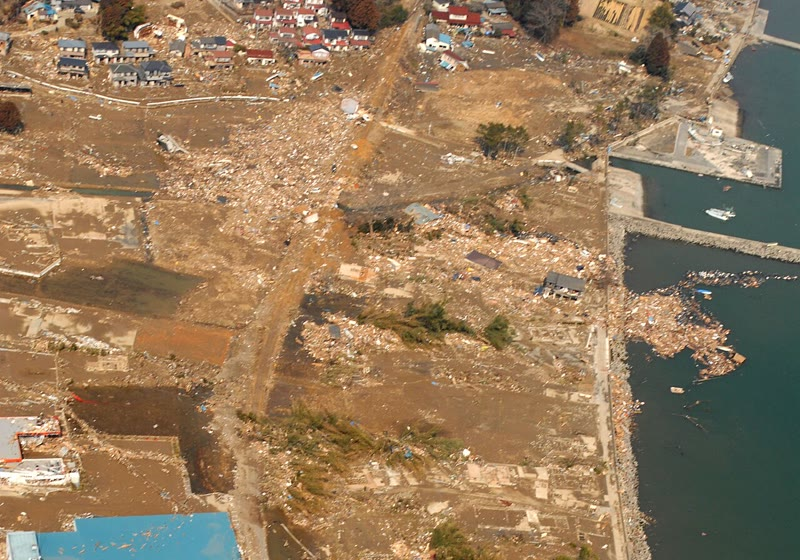
\includegraphics[width=0.78\linewidth]{images/book2/g11-usn-tsunami-kesennuma.jpg}

{\small Le port de pêche de Kesennuma, sur la côte nord-est du Japon, deux
jours après le tsunami du 11~mars 2011. Photographie Dylan McCord, U.S.
Navy (domaine public).}
\end{omfigure}
% ledger: photo:g11-tsunami

\section{Exercices}

\begin{exercise}[$\star$]\label{exo:g11:subduction-zones:1}
Définir la \omterm{def:g11:subduction-zones:subduction}{subduction} et une \omterm{def:g11:subduction-zones:subduction}{zone de subduction}. Quel type de \omterm{def:g11:lithosphere-asthenosphere:lithosphere}{lithosphère}
s'enfonce à une \omterm{def:g11:subduction-zones:subduction}{zone de subduction}, et pourquoi ce type-là~?
\end{exercise}

\begin{exercise}[$\star$]\label{exo:g11:subduction-zones:2}
À l'aide de la carte mondiale des séismes selon leur profondeur~:
(1) nommer trois régions où se produisent des séismes à plus de
\qty{300}{km} de profondeur~; (2) de quel côté d'une fosse se trouvent les
séismes profonds~? (3) Le long de la dorsale médio-atlantique, à quelle
profondeur se produisent les séismes~?
\end{exercise}

\begin{exercise}[$\star$]\label{exo:g11:subduction-zones:3}
Le catalogue contient \num{7031} séismes de magnitude 6 ou plus, dont
\qty{21}{\percent} à plus de \qty{70}{km} de profondeur et
\qty{6.9}{\percent} à plus de \qty{300}{km}. Combien de séismes cela
fait-il dans chaque cas~?
\end{exercise}

\begin{exercise}[$\star$]\label{exo:g11:subduction-zones:4}
Définir le \omterm{def:g11:subduction-zones:eclogite}{schiste bleu} et l'\omterm{def:g11:subduction-zones:eclogite}{éclogite}. Qu'ont-ils tous deux en commun avec
le basalte de la \omterm{def:g11:ocean-ridges:oceanic-lithosphere}{croûte océanique}~? Qu'est-ce qui diffère~?
\end{exercise}

\begin{exercise}[$\star$]\label{exo:g11:subduction-zones:5}
Énumérer dans l'ordre les parties d'une \omterm{def:g11:subduction-zones:subduction}{zone de subduction}, depuis le fond
océanique qui avance vers la fosse jusqu'à l'arrière-arc, en disant en une
ligne ce qui se passe dans chacune.
\end{exercise}

\begin{exercise}[$\star\star$]\label{exo:g11:subduction-zones:6}
Sur la coupe des Andes, la droite qui suit les séismes passe à
\qty{135}{km} de profondeur à \qty{300}{km} de la fosse et à
\qty{508}{km} de profondeur à \qty{800}{km}. Calculer le pendage du \omterm{def:g11:subduction-zones:slab}{panneau
plongeant}.
\end{exercise}

\begin{exercise}[$\star\star$]\label{exo:g11:subduction-zones:7}
Un \omterm{def:g11:subduction-zones:slab}{panneau plongeant} rectiligne part d'une fosse avec un pendage de
\ang{45}. (1) À quelle profondeur se trouve-t-il à \qty{300}{km} de la
fosse~? (2) À quelle distance de la fosse atteint-il \qty{670}{km}~?
(3) Quelle longueur de \omterm{def:g11:subduction-zones:slab}{panneau} se trouve entre la fosse et \qty{670}{km}~?
\end{exercise}

\begin{exercise}[$\star\star$]\label{exo:g11:subduction-zones:8}
Les vitesses moyennes des plaques sont, en millimètres par an~: Cocos 74.6,
Nazca 70.0, Pacifique 65.5, Australie 63.1, mer des Philippines 52.6 (avec
\omterm{def:g11:subduction-zones:slab}{panneau plongeant})~; Arabie 47.6, Somalie 31.0, Nubie 29.2, Eurasie 22.8,
Amérique du Nord 19.8, Antarctique 15.2, Caraïbes 14.9, Amérique du Sud 10.6
(sans). (1) Calculer la moyenne de chaque groupe et leur rapport. (2) Que
cela suggère-t-il sur la force qui met les plaques en mouvement~?
\end{exercise}

\begin{exercise}[$\star\star$]\label{exo:g11:subduction-zones:9}
En 2011, la faille au large du Japon a glissé de 50 à \qty{60}{m} au plus.
La plaque Pacifique se rapproche à \qty{83}{mm} par an. (1) À combien
d'années de mouvement de plaque correspond un glissement de \qty{50}{m},
puis de \qty{60}{m}~? (2) Comparer à la durée écoulée depuis 869, date d'un
possible séisme antérieur de même taille.
\end{exercise}

\begin{exercise}[$\star\star$]\label{exo:g11:subduction-zones:10}
Le fond océanique qui atteint la fosse du Japon a environ 133 millions
d'années, celui qui atteint les Tonga environ 99 et celui qui atteint les
Andes environ 49. (1) À l'aide des lois du \cref{ch:g11:ocean-ridges}
($2500 + 350\sqrt{t}$ pour
$t \le 70$, $6400 - 3200\,e^{-t/62.8}$ au-delà), trouver la profondeur de
chacun. (2) Quelle est la \omterm{def:g11:lithosphere-asthenosphere:lithosphere}{lithosphère} la plus froide et la plus dense~?
\end{exercise}

\begin{exercise}[$\star\star$]\label{exo:g11:subduction-zones:11}
Le basalte de la \omterm{def:g11:ocean-ridges:oceanic-lithosphere}{croûte océanique} a une masse volumique d'environ
\qty{2900}{kg/m^3}, le manteau qui entoure le \omterm{def:g11:subduction-zones:slab}{panneau plongeant}
\qty{3380}{kg/m^3}, et l'\omterm{def:g11:subduction-zones:eclogite}{éclogite} est plus dense que le manteau de
\qty{6}{\percent}. (1) Trouver la masse volumique de l'\omterm{def:g11:subduction-zones:eclogite}{éclogite}. (2) De quel
pourcentage la masse volumique de la croûte augmente-t-elle quand elle se
transforme en \omterm{def:g11:subduction-zones:eclogite}{éclogite}~? (3) Avant et après, la croûte est-elle plus légère
ou plus dense que le manteau, et de combien~?
\end{exercise}

\begin{exercise}[$\star\star\star$]\label{exo:g11:subduction-zones:12}
La chaleur se propage par conduction sur une distance d'environ
$\sqrt{\kappa t}$ en un temps $t$, avec $\kappa = \qty{1e-6}{m^2/s}$ pour
la roche. (1) Calculer cette distance pour 6 millions d'années
($1~\text{an} \approx \qty{3.16e7}{s}$). (2) La comparer à l'épaisseur d'un
\omterm{def:g11:subduction-zones:slab}{panneau plongeant}, environ \qty{100}{km}. (3) Expliquer pourquoi des séismes
peuvent se produire à l'intérieur d'un \omterm{def:g11:subduction-zones:slab}{panneau plongeant} à \qty{600}{km}
alors que le manteau qui l'entoure s'écoule.
\end{exercise}
% ledger: england:kelvin (kappa 1e-6 m2/s)

\begin{exercise}[$\star\star\star$]\label{exo:g11:subduction-zones:13}
Sous les Andes à \ang{21}~Sud, la droite de la coupe atteint
\qty{670}{km} à \qty{1017}{km} de la fosse, et les plaques convergent à
\qty{64}{mm} par an. (1) Estimer la longueur du \omterm{def:g11:subduction-zones:slab}{panneau plongeant} depuis la
fosse jusqu'à \qty{670}{km}. (2) Combien de temps un morceau de fond
océanique met-il pour atteindre \qty{670}{km}~? (3) Comparer aux Tonga, où
le même trajet prend environ 6 millions d'années.
\end{exercise}

\begin{exercise}[$\star\star\star$]\label{exo:g11:subduction-zones:14}
On considère un \omterm{def:g11:subduction-zones:slab}{panneau plongeant} épais de \qty{100}{km}, plus dense que le
manteau qui l'entoure de \qty{36}{kg/m^3} en moyenne, et long de
\qty{1000}{km}, sous une fosse. (1) Calculer l'excès de masse du \omterm{def:g11:subduction-zones:slab}{panneau}
pour chaque mètre de fosse. (2) Calculer son poids, avec
$g = \qty{9.8}{m/s^2}$. (3) Pourquoi cette force peut-elle tirer toute la
plaque~?
\end{exercise}

\begin{exercise}[$\star\star\star$]\label{exo:g11:subduction-zones:15}
Le long de la fosse des Tonga, le modèle PB2002 donne une convergence de
\qty{104}{mm} par an à \ang{23.6}~Sud et de \qty{237}{mm} par an à
\ang{16.5}~Sud. (1) Quelle distance sépare les deux points, le long d'un
méridien ($\ang{1} \approx \qty{111}{km}$)~? (2) De combien la vitesse
augmente-t-elle par centaine de kilomètres~? (3) La plaque Pacifique se
déplace à peu près à la même vitesse aux deux points. Que doit faire
l'autre bord de la fosse, l'arc des Tonga~?
\end{exercise}

\section{Problème~: le panneau plongeant des Tonga}

\begin{problem}[{Problème du week-end --- de la fosse jusqu'à \qty{670}{km}}]
\label{pb:g11:subduction-zones:1}
% values: tonga fit -23.568 + 0.91068 x; tonga_rate 168.0 mm/yr; tonga_age 98.8;
% x670 761.6; path 1014; time 6.04 Myr; tonga_maxdepth 670.8 (slab_sections.py);
% MKEA 69 mm/yr (plate_velocities.py); kappa england:kelvin; eclogite hacker03:eclogite
Sous la fosse des Tonga, la plaque Pacifique s'enfonce vers l'ouest. On
utilise la coupe des Tonga de ce chapitre, dont la droite a pour équation
$z = -24 + 0.91\,x$ (les deux en
kilomètres, $x$ étant mesuré depuis la fosse vers l'arc).

\medskip
\noindent\textbf{Partie I --- La coupe de séismes.}
\begin{enumerate}
  \item À quelle profondeur se trouve le séisme le plus profond de la
        coupe~?
  \item Pourquoi n'y a-t-il pas de séismes profonds du côté océanique de la
        fosse~?
  \item Calculer la profondeur de la droite en $x = 300$ et en $x = 700$,
        puis le pendage du \omterm{def:g11:subduction-zones:slab}{panneau plongeant}.
  \item À quelle distance horizontale de la fosse le \omterm{def:g11:subduction-zones:slab}{panneau plongeant}
        est-il à \qty{100}{km} de profondeur~? Et à \qty{400}{km}~?
  \item La droite passe \qty{24}{km} au-dessus de la fosse en $x = 0$.
        Qu'est-ce que cela indique sur la forme du \omterm{def:g11:subduction-zones:slab}{panneau plongeant} près
        de la fosse~?
\end{enumerate}

\medskip
\noindent\textbf{Partie II --- La convergence.}
\begin{enumerate}[resume]
  \item Les plaques convergent de part et d'autre de la fosse à environ
        \qty{168}{mm} par an. Convertir en centimètres par an et en
        kilomètres par million d'années.
  \item La plaque Pacifique se déplace au-dessus d'Hawaï à environ
        \qty{69}{mm} par an. Combien de fois la convergence aux Tonga
        est-elle plus rapide~?
  \item À l'aide de la somme des vitesses relatives, expliquer comment la
        convergence peut dépasser la vitesse de la plaque Pacifique.
  \item Le fond qui atteint la fosse a environ 99 millions d'années. À
        quelle profondeur se trouve-t-il (loi exponentielle du
        \cref{ch:g11:ocean-ridges})~?
  \item Pourquoi une telle \omterm{def:g11:lithosphere-asthenosphere:lithosphere}{lithosphère} peut-elle s'enfoncer d'elle-même~?
\end{enumerate}

\medskip
\noindent\textbf{Partie III --- Jusqu'à \qty{670}{km}.}
\begin{enumerate}[resume]
  \item À quelle distance horizontale de la fosse la droite atteint-elle
        \qty{670}{km}~?
  \item Estimer la longueur du \omterm{def:g11:subduction-zones:slab}{panneau plongeant} depuis la fosse jusqu'à
        ce point, en le supposant rectiligne.
  \item Combien de temps un morceau de fond océanique met-il pour parcourir
        cette longueur à \qty{168}{mm} par an~?
  \item Combien de temps mettrait-il aux \qty{69}{mm} par an de la plaque
        Pacifique au-dessus d'Hawaï~?
  \item En chemin, la croûte du \omterm{def:g11:subduction-zones:slab}{panneau plongeant} se transforme en
        \omterm{def:g11:subduction-zones:eclogite}{éclogite}, plus dense de \qty{6}{\percent} que le manteau à
        \qty{3380}{kg/m^3}. Quelle est sa masse volumique, et qu'est-ce que
        cela change pour le \omterm{def:g11:subduction-zones:slab}{panneau plongeant}~?
\end{enumerate}

\medskip
\noindent\textbf{Partie IV --- Un panneau froid dans un manteau chaud.}
\begin{enumerate}[resume]
  \item Pendant la durée de la question~13, la chaleur se propage par
        conduction sur environ $\sqrt{\kappa t}$, avec
        $\kappa = \qty{1e-6}{m^2/s}$. Calculer cette distance.
  \item La comparer à l'épaisseur du \omterm{def:g11:subduction-zones:slab}{panneau plongeant}, environ
        \qty{100}{km}. Le \omterm{def:g11:subduction-zones:slab}{panneau} est-il encore froid à l'intérieur quand il
        atteint \qty{670}{km}~?
  \item Pourquoi cela explique-t-il les séismes à \qty{600}{km} et plus sous
        les Tonga~?
  \item Quel changement dans le manteau les ondes sismiques ont-elles
        révélé vers \qty{670}{km} (\cref{ch:g11:seismic-structure})~?
  \item Conclure~: combien de temps le fond océanique du Pacifique met-il
        pour descendre de la fosse des Tonga jusqu'à \qty{670}{km}~?
\end{enumerate}
\end{problem}
